\documentclass[aspectratio=169]{beamer}

\usetheme{default}
\setbeamertemplate{navigation symbols}{}
\setbeamertemplate{itemize item}{\color{black}\textbullet}
\setbeamertemplate{itemize subitem}{\color{black}\textbullet}
\usepackage{xcolor}
\usepackage{tikz}
\usetikzlibrary{shapes,arrows,positioning}
\definecolor{navy}{RGB}{0, 0, 128}
\definecolor{hi}{RGB}{220, 20, 60}

% TikZ styles
\tikzstyle{decision} = [ellipse, draw, text width=4em, text centered, node distance=3cm]
\tikzstyle{process} = [rectangle, draw, text width=4em, text centered, rounded corners, minimum height=2em, node distance=2.75cm]
\tikzstyle{line} = [draw, -latex']

\begin{document}

\begin{frame}

\only<1>{
\begin{center}
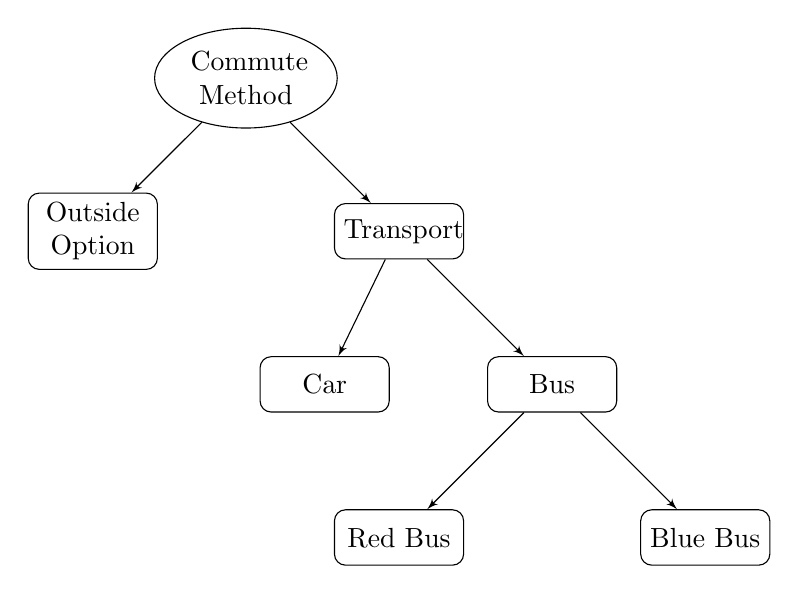
\begin{tikzpicture}[node distance=0.5cm, auto]
    \node [decision] (choice) {Commute Method};
    \node [process, below right of=choice] (transport) {Transport};
    \node [process, below left of=choice] (outside) {Outside Option};
    \node [process, below left of=transport, xshift=1cm] (car) {Car};
    \node [process, below right of=transport] (bus) {Bus};
    \node [process, below left of=bus] (redbus) {Red Bus};
    \node [process, below right of=bus] (bluebus) {Blue Bus};
    
    \path [line] (choice) -- (transport);
    \path [line] (choice) -- (outside);
    \path [line] (transport) -- (car);
    \path [line] (transport) -- (bus);
    \path [line] (bus) -- (redbus);
    \path [line] (bus) -- (bluebus);
\end{tikzpicture}
\end{center}
}


\only<2>{
\begin{center}
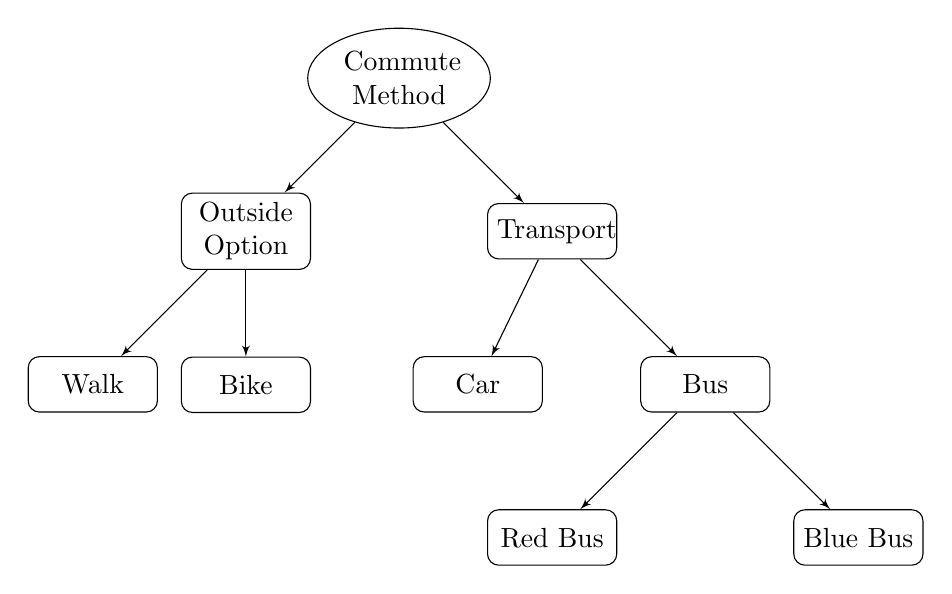
\begin{tikzpicture}[node distance=0.5cm, auto]
    \node [decision] (choice) {Commute Method};
    \node [process, below right of=choice] (transport) {Transport};
    \node [process, below left of=choice] (outside) {Outside Option};
    \node [process, below left of=outside] (walk) {Walk};    
    \node [process, below of=outside, yshift=0.8cm] (bike) {Bike};
    \node [process, below left of=transport, xshift=1cm] (car) {Car};
    \node [process, below right of=transport] (bus) {Bus};
    \node [process, below left of=bus] (redbus) {Red Bus};
    \node [process, below right of=bus] (bluebus) {Blue Bus};
    
    \path [line] (choice) -- (transport);
    \path [line] (choice) -- (outside);
    \path [line] (outside) -- (walk);
    \path [line] (outside) -- (bike);
    \path [line] (transport) -- (car);
    \path [line] (transport) -- (bus);
    \path [line] (bus) -- (redbus);
    \path [line] (bus) -- (bluebus);
\end{tikzpicture}
\end{center}
}

\end{frame}

\begin{frame}
\includegraphics[width=\textwidth]{EAScover.jpg}
\end{frame}


\begin{frame}

\begin{center}
Policy Question: Is Essential Air Service still essential?
\end{center}

\begin{itemize}
\item[]
\item Created in 1978 as temporary transition program
\item[]
\item Now costs \$540M+ annually 
\item[]
\item Serves 107 communities
\item[]
\item Original rationale: prevent rural isolation post-deregulation of airlines
\end{itemize}

\end{frame}



\begin{frame}
\centering
\includegraphics[width=.9\textwidth]{EASfig2.jpg}
\end{frame}

\begin{frame}

\begin{center}
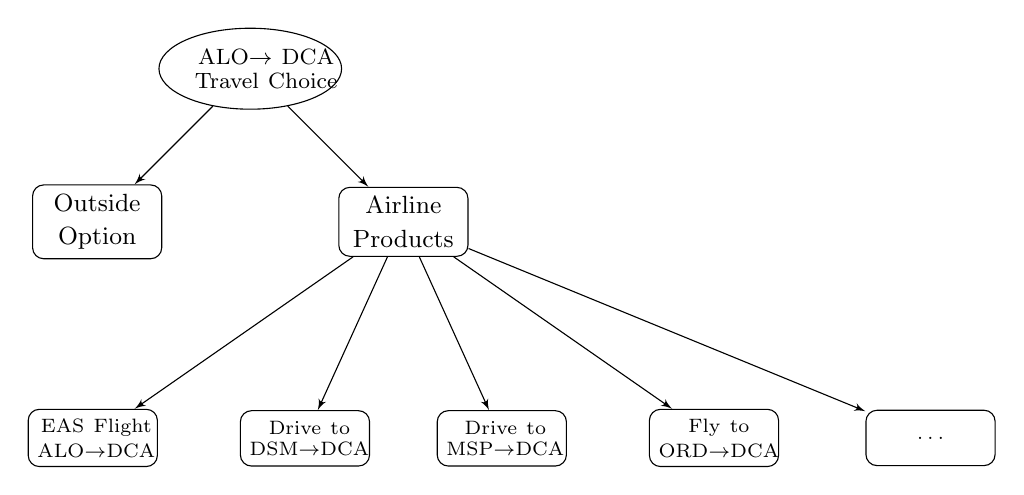
\begin{tikzpicture}[node distance=2.5cm, auto]
    \node [decision] (choice) {\footnotesize \shortstack{ALO$\rightarrow$ DCA \\ Travel Choice}};
    \node [process, below right of=choice] (fly) {\small Airline Products};
    \node [process, below left of=choice] (outside) {\small Outside Option};
    \node [process, below left of=fly, xshift=-2cm, yshift=-0.8cm] (eas) {\scriptsize \shortstack{EAS Flight \\ ALO$\rightarrow$DCA}};
    \node [process, below of=fly, xshift=-1.25cm] (dsm) {\scriptsize \shortstack{Drive to \\ DSM$\rightarrow$DCA}};
    \node [process, below right of=fly, xshift=2cm, yshift=-0.8cm] (ord) {\scriptsize \shortstack{Fly to \\ ORD$\rightarrow$DCA}};
    \node [process, below right of=fly, xshift=4.75cm, yshift=-0.8cm] (dots) {\scriptsize $\ldots$};
    \node [process, below of=fly, xshift=1.25cm] (msp) {\scriptsize \shortstack{Drive to \\ MSP$\rightarrow$DCA}};
    
    \path [line] (choice) -- (fly);
    \path [line] (choice) -- (outside);
    \path [line] (fly) -- (eas);
    \path [line] (fly) -- (dsm);
    \path [line] (fly) -- (ord);
    \path [line] (fly) -- (dots);
    \path [line] (fly) -- (msp);
\end{tikzpicture}
\end{center}
\end{frame}

\begin{frame}
\centering
\includegraphics[width=.9\textwidth]{EASutilityfn.jpg}
\end{frame}

\begin{frame}
\centering
\includegraphics[width=.9\textwidth]{EASestimates.jpg}
\end{frame}

\begin{frame}
\centering
\includegraphics[width=.9\textwidth]{EASconsumersurplus.jpg}
\end{frame}

\begin{frame}
\centering
\includegraphics[width=.9\textwidth]{EAStable3.jpg}
\end{frame}


\begin{frame}
\centering
\includegraphics[width=.9\textwidth]{EASfig6.jpg}

\bigskip{}

Counterfactual: remove EAS subsidies and see which airlines would retain service
\end{frame}






\end{document}